\documentclass[12pt,letterpaper]{article}

% Evidencia: GA4-220501095-AA2-EV05
% Compilar con LaTeX Workshop o: latexmk -pdf GA4-220501095-AA2-EV05.tex
% El contenido usa caracteres ASCII para evitar problemas de codificacion.

\usepackage[spanish,es-nodecimaldot,shorthands=off]{babel}
\usepackage[T1]{fontenc}
\usepackage[utf8]{inputenc}
\usepackage{lmodern}
\usepackage{geometry}
\usepackage{setspace}
\usepackage{array}
\usepackage{longtable}
\usepackage{enumitem}
\usepackage{xcolor}
\usepackage{titlesec}
\usepackage{fancyhdr}
\usepackage{graphicx}
\usepackage{pdflscape}
\usepackage{hyperref}

% ==================== DATOS CONFIGURABLES ====================
\newcommand{\institucion}{Servicio Nacional de Aprendizaje -- SENA}
\newcommand{\programa}{Analisis y Desarrollo de Software}
\newcommand{\tituloTrabajo}{Arquitectura de software de acuerdo con el patron de diseno seleccionado}
\newcommand{\codigoEvidencia}{GA4-220501095-AA2-EV05}
\newcommand{\nombreProyecto}{Sistema de Gestion de Citas SAC}
\newcommand{\aprendiz}{Kevin Andres Granados Daza}
\newcommand{\instructor}{[Jesus Ramirez]}
\newcommand{\ficha}{[3389015]}
\newcommand{\ciudad}{Bogota D. C.}
\newcommand{\fechaEntrega}{[25 de septiembre de 2026]}
% ==============================================================

\geometry{top=2.54cm,bottom=2.54cm,left=2.54cm,right=2.54cm}
\onehalfspacing
\setlength{\parindent}{1.27cm}
\setlength{\parskip}{0pt}
\setlength{\headheight}{15pt}

\pagestyle{fancy}
\fancyhf{}
\fancyhead[L]{\codigoEvidencia}
\fancyhead[R]{\thepage}
\renewcommand{\headrulewidth}{0pt}

\titleformat{\section}{\normalfont\Large\bfseries\centering}{\thesection.}{0.5em}{}
\titleformat{\subsection}{\normalfont\large\bfseries}{\thesubsection.}{0.5em}{}

\begin{document}

\begin{titlepage}
    \centering
    \vspace*{2.5cm}
    {\Large \tituloTrabajo\par}
    \vspace{0.8cm}
    {\large Proyecto: \nombreProyecto\par}
    \vfill
    {\large \aprendiz\par}
    \vspace{1.5cm}
    {\large \institucion\par}
    {\large \programa\par}
    \vspace{1cm}
    {\large Evidencia: \codigoEvidencia\par}
    \vspace{1cm}
    {\large Instructor(a): \instructor\par}
    {\large Ficha: \ficha\par}
    \vfill
    {\large \ciudad\par}
    {\large \fechaEntrega\par}
\end{titlepage}

\section{Introduccion}

La arquitectura de software define la organizacion general de una aplicacion y establece la forma en que sus componentes interactuan entre si. Una arquitectura adecuada permite que el codigo fuente sea mas claro, mantenible, escalable y seguro. Ademas, facilita que el equipo de desarrollo pueda comprender las responsabilidades de cada modulo y realizar cambios sin afectar innecesariamente el resto del sistema.

El presente documento desarrolla la arquitectura propuesta para el proyecto \nombreProyecto. Este sistema se plantea como una aplicacion web que permite registrar usuarios, administrar horarios, agendar, cancelar y reprogramar citas, asi como confirmar, rechazar y hacer seguimiento a las solicitudes realizadas.

Para la solucion se propone una arquitectura web por capas basada en el patron Modelo Vista Controlador, complementada con patrones como Service Layer, Repository, Factory Method, Observer y Data Transfer Object. Tambien se presentan la vista de componentes, la vista de despliegue y las herramientas necesarias para optimizar los procesos de desarrollo, pruebas, documentacion y publicacion de la aplicacion.

\section{Descripcion del sistema}

\subsection{Sistema de Gestion de Citas SAC}

El Sistema de Gestion de Citas SAC es una aplicacion web orientada a centralizar la administracion de citas y horarios de atencion. El sistema permite que un usuario se registre, inicie sesion, consulte horarios disponibles, solicite una cita, cancele una cita o la reprograme. Por otra parte, el administrador puede gestionar la disponibilidad de horarios, visualizar las solicitudes, confirmar o rechazar citas y controlar los estados de cada proceso.

La solucion busca disminuir actividades manuales, evitar cruces de horario, conservar la informacion de manera persistente y mejorar la trazabilidad de las acciones realizadas. El sistema tambien puede generar notificaciones cuando una cita es creada, confirmada, rechazada, cancelada o reprogramada.

\subsection{Requisitos arquitectonicos principales}

La arquitectura debe responder a las siguientes condiciones del proyecto:

\begin{itemize}[leftmargin=1.2cm]
    \item Acceso mediante una aplicacion web responsiva desde navegadores modernos.
    \item Separacion entre interfaz de usuario, logica de negocio y persistencia de datos.
    \item Autenticacion y control de acceso de acuerdo con los roles de usuario y administrador.
    \item Validacion de disponibilidad antes de registrar una cita.
    \item Persistencia de usuarios, horarios, citas, estados, historial y notificaciones.
    \item Capacidad para registrar los cambios realizados sobre una cita.
    \item Facilidad para ejecutar pruebas, corregir errores y ampliar funcionalidades futuras.
    \item Posibilidad de desplegar la aplicacion en infraestructura en la nube o en un servidor virtual.
\end{itemize}

\section{Arquitectura seleccionada}

\subsection{Arquitectura web por capas}

Para el Sistema de Gestion de Citas SAC se selecciona una arquitectura web por capas. Este enfoque divide la aplicacion en componentes con responsabilidades especificas y permite que cada parte evolucione sin afectar de forma directa las demas.

La arquitectura propuesta se organiza en las siguientes capas:

\begin{longtable}{|p{3.6cm}|p{4.3cm}|p{6.1cm}|}
\hline
\textbf{Capa} & \textbf{Componentes principales} & \textbf{Responsabilidad} \\
\hline
\endfirsthead
\hline
\textbf{Capa} & \textbf{Componentes principales} & \textbf{Responsabilidad} \\
\hline
\endhead
\hline
\endfoot
\hline
\endlastfoot

Presentacion & Frontend web, formularios, paneles, vistas y validaciones basicas. & Permite la interaccion de Usuario y Administrador con el sistema mediante navegador web. \\
\hline

API y controladores & API REST, rutas, controladores y autenticacion. & Recibe solicitudes HTTP, valida datos iniciales, controla acceso y dirige cada solicitud al servicio correspondiente. \\
\hline

Logica de negocio & Servicios de usuario, citas, horarios, autenticacion y notificaciones. & Aplica reglas del negocio, controla transacciones y coordina las operaciones entre modelos y repositorios. \\
\hline

Dominio & Usuario, Administrador, Rol, Cita, Horario, HistorialCita, Notificacion y EstadoCita. & Representa las entidades principales del problema y sus comportamientos orientados a objetos. \\
\hline

Persistencia & Repositorios, ORM y base de datos relacional. & Encapsula operaciones de consulta, almacenamiento, actualizacion y eliminacion de datos. \\
\hline

Infraestructura externa & Servicio de correo, almacenamiento, servidor y monitoreo. & Permite integrar servicios externos requeridos para notificaciones, despliegue y operacion del sistema. \\
\hline
\end{longtable}

Este modelo permite que la interfaz web no acceda directamente a la base de datos. Las solicitudes pasan por la API REST, los controladores y los servicios de negocio. Posteriormente, los repositorios realizan las operaciones necesarias sobre la base de datos. Esta separacion favorece el mantenimiento y reduce el acoplamiento entre componentes.

\subsection{Flujo general de una solicitud}

El siguiente flujo describe de manera general como se procesa una accion dentro del sistema:

\begin{enumerate}[leftmargin=1.2cm]
    \item El usuario realiza una accion desde el frontend web, por ejemplo solicitar una cita.
    \item El frontend envía una solicitud HTTPS en formato JSON a la API REST.
    \item La API valida autenticacion, rol y formato de los datos recibidos.
    \item El controlador correspondiente delega la operacion al ServicioCita.
    \item El servicio aplica las reglas del negocio, por ejemplo verificar que el horario este disponible.
    \item El servicio utiliza los repositorios para consultar o actualizar los datos necesarios.
    \item La base de datos almacena la informacion de la cita y del historial de cambios.
    \item Si ocurre un cambio relevante, el ServicioNotificacion prepara y envia un mensaje al usuario.
    \item La API devuelve una respuesta JSON y el frontend muestra el resultado de la operacion.
\end{enumerate}

\section{Patrones de diseno aplicados}

Los patrones de diseno permiten aplicar soluciones reutilizables a problemas frecuentes de organizacion del software. En este proyecto se utiliza MVC como patron principal de organizacion, complementado con otros patrones que ayudan a reducir duplicacion, desacoplar componentes y mantener las reglas de negocio centralizadas.

\subsection{Modelo Vista Controlador}

El patron Modelo Vista Controlador, conocido como MVC, divide la aplicacion en tres partes principales:

\begin{itemize}[leftmargin=1.2cm]
    \item \textbf{Modelo:} representa los datos y reglas del dominio. En el SAC incluye Usuario, Administrador, Cita, Horario, HistorialCita y Notificacion.
    \item \textbf{Vista:} corresponde a las paginas, formularios, paneles y elementos visuales que utiliza el usuario desde el navegador.
    \item \textbf{Controlador:} recibe las solicitudes del usuario, valida la informacion inicial y coordina la comunicacion entre vista y servicios de negocio.
\end{itemize}

MVC permite separar la interfaz de usuario de las reglas del negocio. Por ejemplo, una modificacion en el formulario para agendar citas no debe obligar a cambiar la logica que valida disponibilidad ni las consultas de base de datos.

\subsection{Service Layer}

El patron Service Layer centraliza las reglas del negocio en servicios especializados. En lugar de colocar toda la logica dentro de los controladores, el sistema utiliza componentes como ServicioAutenticacion, ServicioUsuario, ServicioCita, ServicioHorario y ServicioNotificacion.

Por ejemplo, ServicioCita puede verificar disponibilidad, crear una cita, actualizar el horario, registrar el cambio en HistorialCita y generar una notificacion. Al centralizar estas acciones se evita repetir la misma logica en varios controladores o pantallas.

\subsection{Repository}

El patron Repository separa la logica de acceso a datos de la logica de negocio. Cada repositorio administra las operaciones de una entidad o grupo de entidades, por ejemplo RepositorioUsuario, RepositorioCita, RepositorioHorario y RepositorioNotificacion.

Los servicios no necesitan conocer los detalles de SQL ni de la conexion a la base de datos. Solo solicitan operaciones como buscar usuario por correo, consultar horarios disponibles, guardar una cita o actualizar el estado de una solicitud. Esto facilita realizar pruebas y modificar la tecnologia de persistencia en el futuro.

\subsection{Factory Method}

El patron Factory Method permite centralizar la creacion de objetos relacionados. En el Sistema de Gestion de Citas SAC puede utilizarse para crear notificaciones de diferentes tipos: confirmacion, rechazo, cancelacion, reprogramacion o recordatorio.

En lugar de crear cada notificacion de forma repetida en diferentes partes del codigo, una fabrica puede recibir el tipo de evento y construir el mensaje correspondiente. Esto reduce duplicacion y facilita agregar nuevos tipos de notificacion.

\subsection{Observer}

El patron Observer permite que uno o varios componentes sean informados cuando cambia el estado de un objeto. En este proyecto, una cita puede actuar como origen del evento. Cuando una cita cambia a confirmada, rechazada, cancelada o reprogramada, el sistema puede notificar al ServicioNotificacion para que genere el mensaje adecuado.

Este patron evita que la clase Cita tenga que conocer directamente los detalles del envio de correos o mensajes. La clase se enfoca en su estado, mientras que los observadores reaccionan a los cambios relevantes.

\subsection{Data Transfer Object}

El patron Data Transfer Object, conocido como DTO, permite transportar informacion controlada entre el frontend y la API REST. Por ejemplo, para crear una cita se puede utilizar un objeto SolicitudCitaDTO con los datos necesarios, como identificador de horario y observacion.

El uso de DTO evita exponer directamente todas las propiedades internas de las entidades. Tambien facilita validar los datos de entrada y construir respuestas consistentes para el frontend.

\begin{longtable}{|p{3.4cm}|p{4.3cm}|p{6.3cm}|}
\hline
\textbf{Patron} & \textbf{Aplicacion en el SAC} & \textbf{Beneficio principal} \\
\hline
\endfirsthead
\hline
\textbf{Patron} & \textbf{Aplicacion en el SAC} & \textbf{Beneficio principal} \\
\hline
\endhead
\hline
\endfoot
\hline
\endlastfoot

MVC & Separa modelos, vistas y controladores. & Reduce acoplamiento entre interfaz, logica y datos. \\
\hline

Service Layer & Centraliza reglas de usuarios, citas, horarios y notificaciones. & Evita duplicacion de logica de negocio. \\
\hline

Repository & Encapsula el acceso a usuarios, horarios, citas y notificaciones. & Facilita pruebas y cambios en persistencia. \\
\hline

Factory Method & Crea notificaciones segun el tipo de evento. & Centraliza la creacion de objetos similares. \\
\hline

Observer & Reacciona ante cambios de estado de una cita. & Desacopla la gestion de citas del envio de notificaciones. \\
\hline

DTO & Transfiere datos controlados entre frontend y API. & Mejora validacion y evita exponer datos internos. \\
\hline
\end{longtable}

\section{Vista de componentes}

La vista de componentes permite observar el sistema en una fase avanzada del ciclo de vida. Esta vista muestra los modulos principales, sus responsabilidades y las dependencias entre ellos. Para el Sistema de Gestion de Citas SAC se identifican componentes de presentacion, aplicacion, dominio, persistencia e integracion externa.

% IMPORTANTE:
% Guarda la primera imagen como: diagrama_componentes_sac.png
% La imagen debe estar en la misma carpeta que este archivo .tex.


\begin{figure}[htbp]
    \centering
    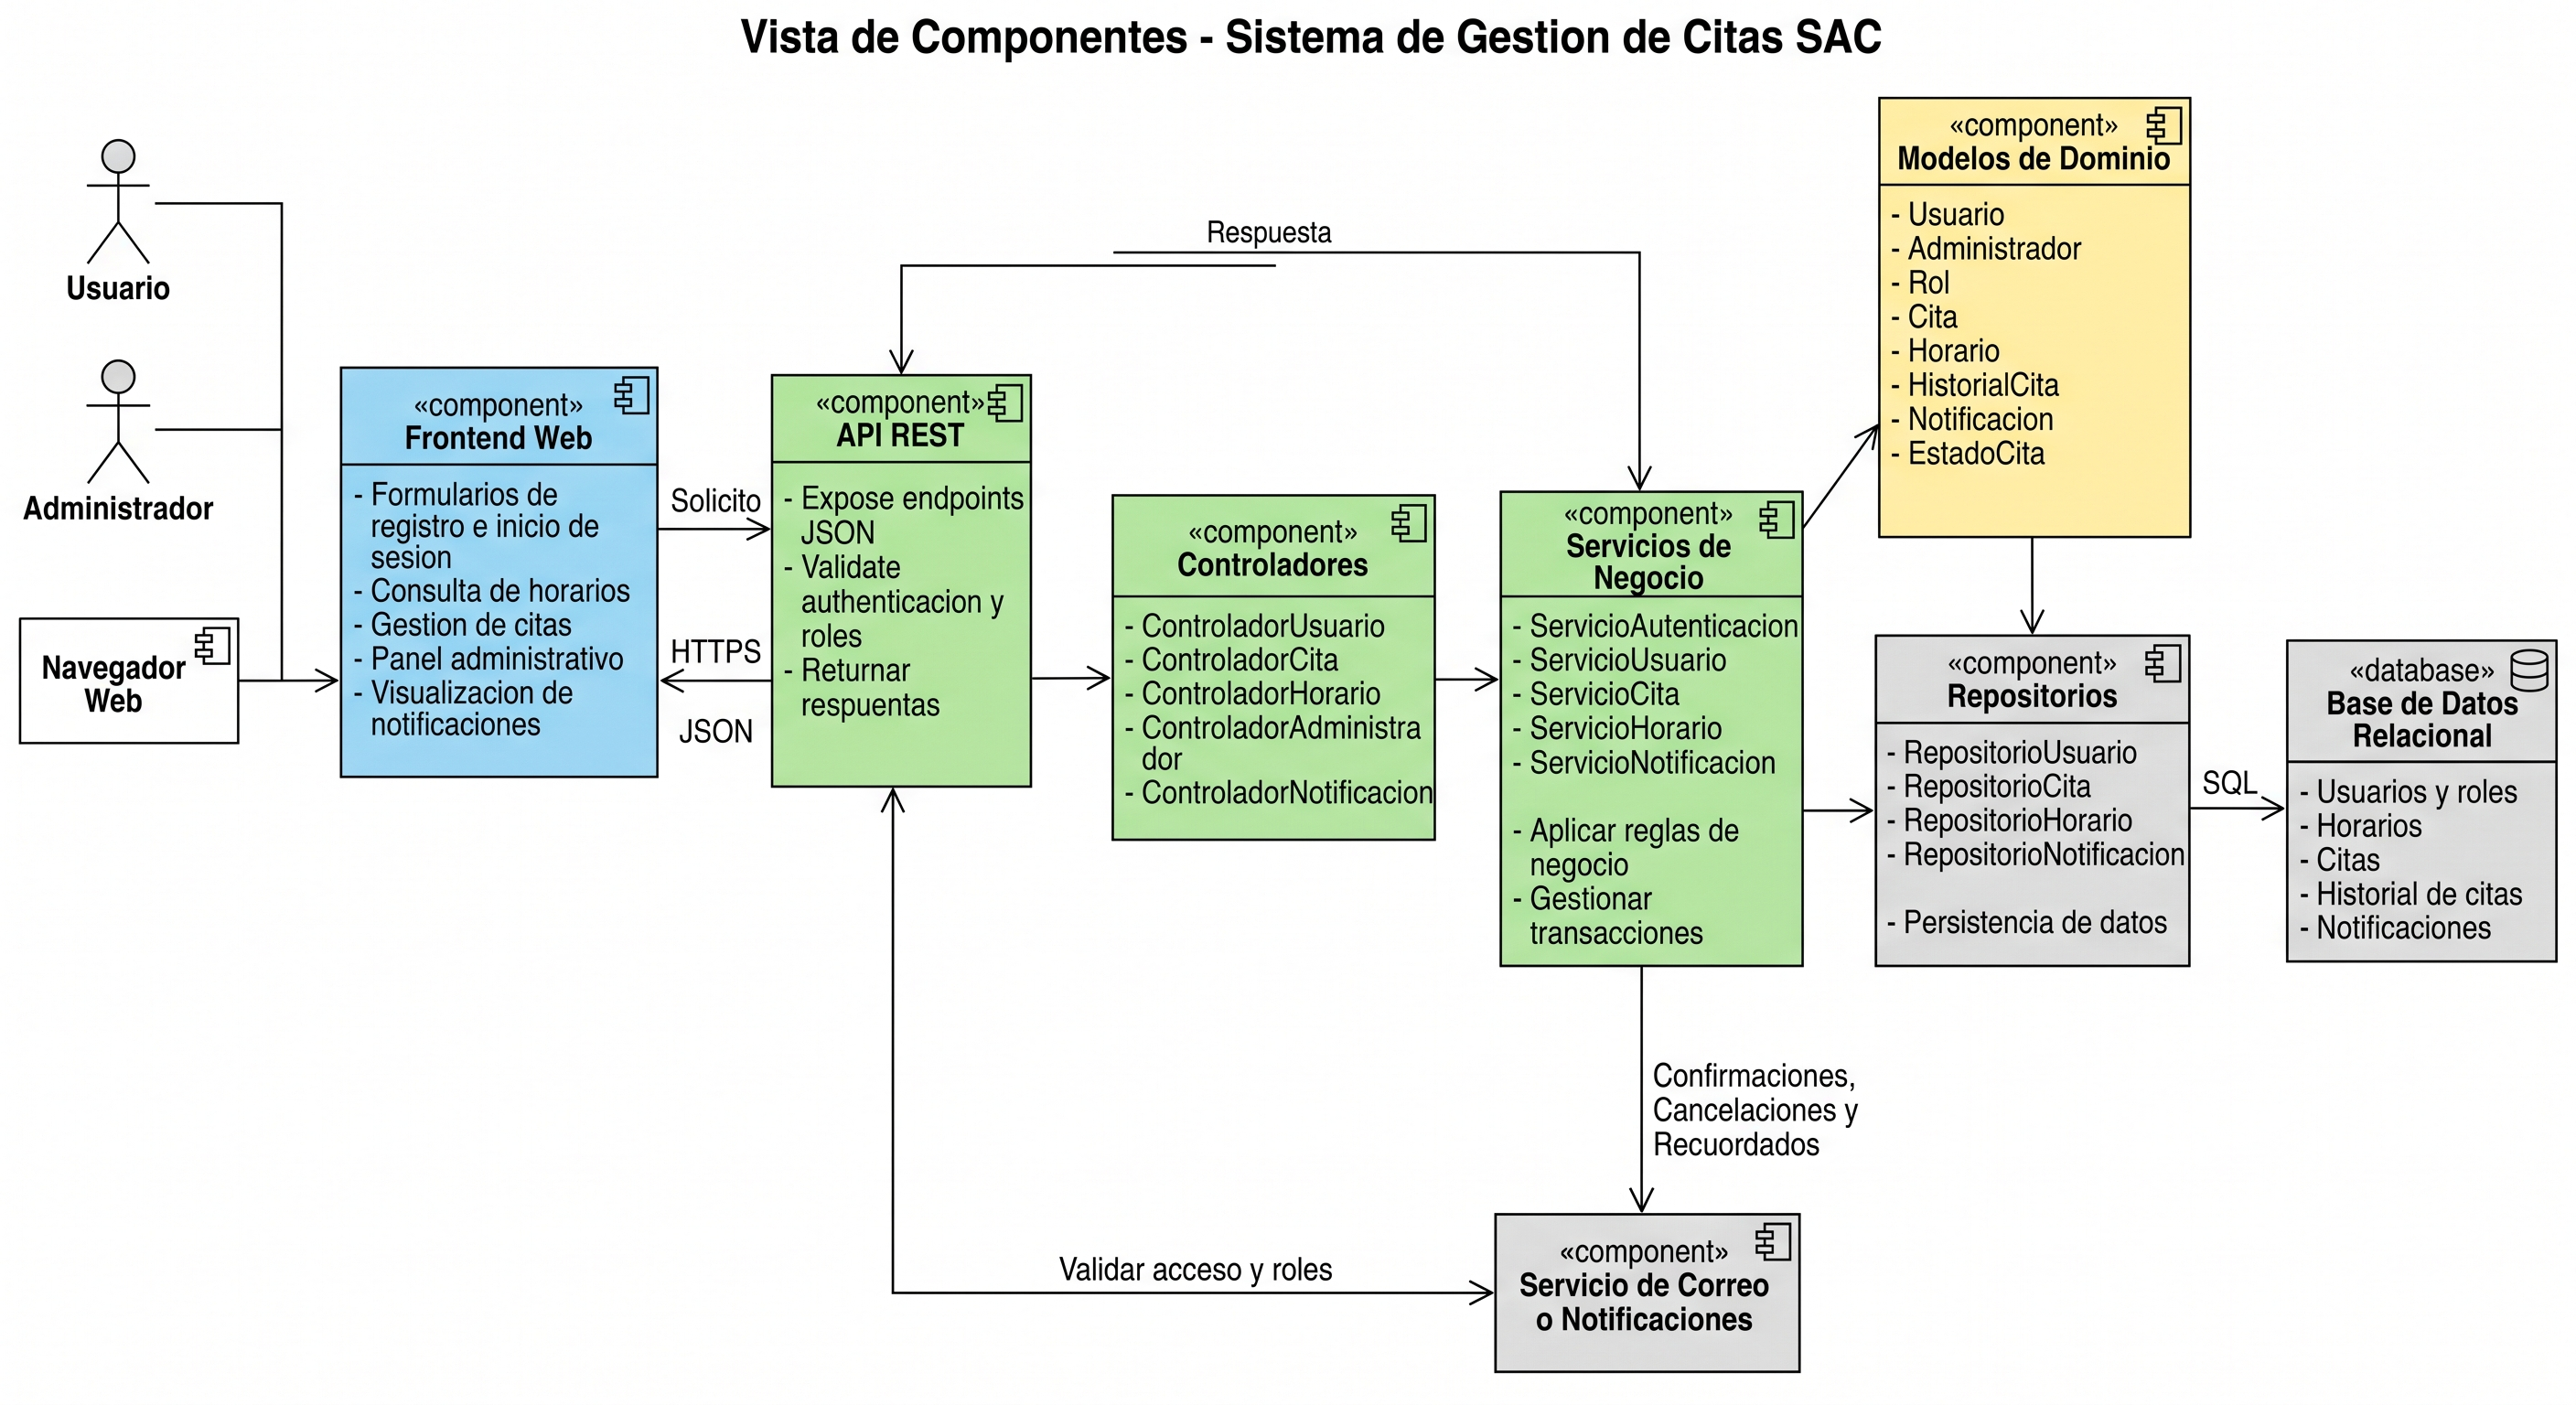
\includegraphics[width=0.9\textwidth]{diagrama_componentes_sac.jpg}
    \caption{Vista de componentes del Sistema de Gestion de Citas SAC.}
    \label{fig:componentes-sac}
\end{figure}



Como se observa en la Figura~\ref{fig:componentes-sac}, Usuario y Administrador interactuan con el sistema mediante el navegador web. El Frontend Web consume los servicios expuestos por la API REST. La API delega el procesamiento a los controladores, y estos utilizan los servicios de negocio para aplicar las reglas del sistema.

Los servicios de negocio utilizan los modelos del dominio y los repositorios. Los repositorios se encargan de acceder a la base de datos relacional. Por otra parte, ServicioCita puede utilizar ServicioNotificacion cuando se registra un cambio relevante en una solicitud. ServicioNotificacion se comunica con un servicio externo de correo o mensajeria para enviar confirmaciones y avisos.

\section{Vista de despliegue}

La vista de despliegue representa las condiciones necesarias para implantar la solucion informatica. Esta vista identifica los dispositivos de usuario, la red, el servidor de aplicacion, el servidor de base de datos y los servicios externos que participan en la operacion del sistema.

% IMPORTANTE:
% Guarda la segunda imagen como: diagrama_despliegue_sac.png
% La imagen debe estar en la misma carpeta que este archivo .tex.



\begin{figure}[htbp]
    \centering
    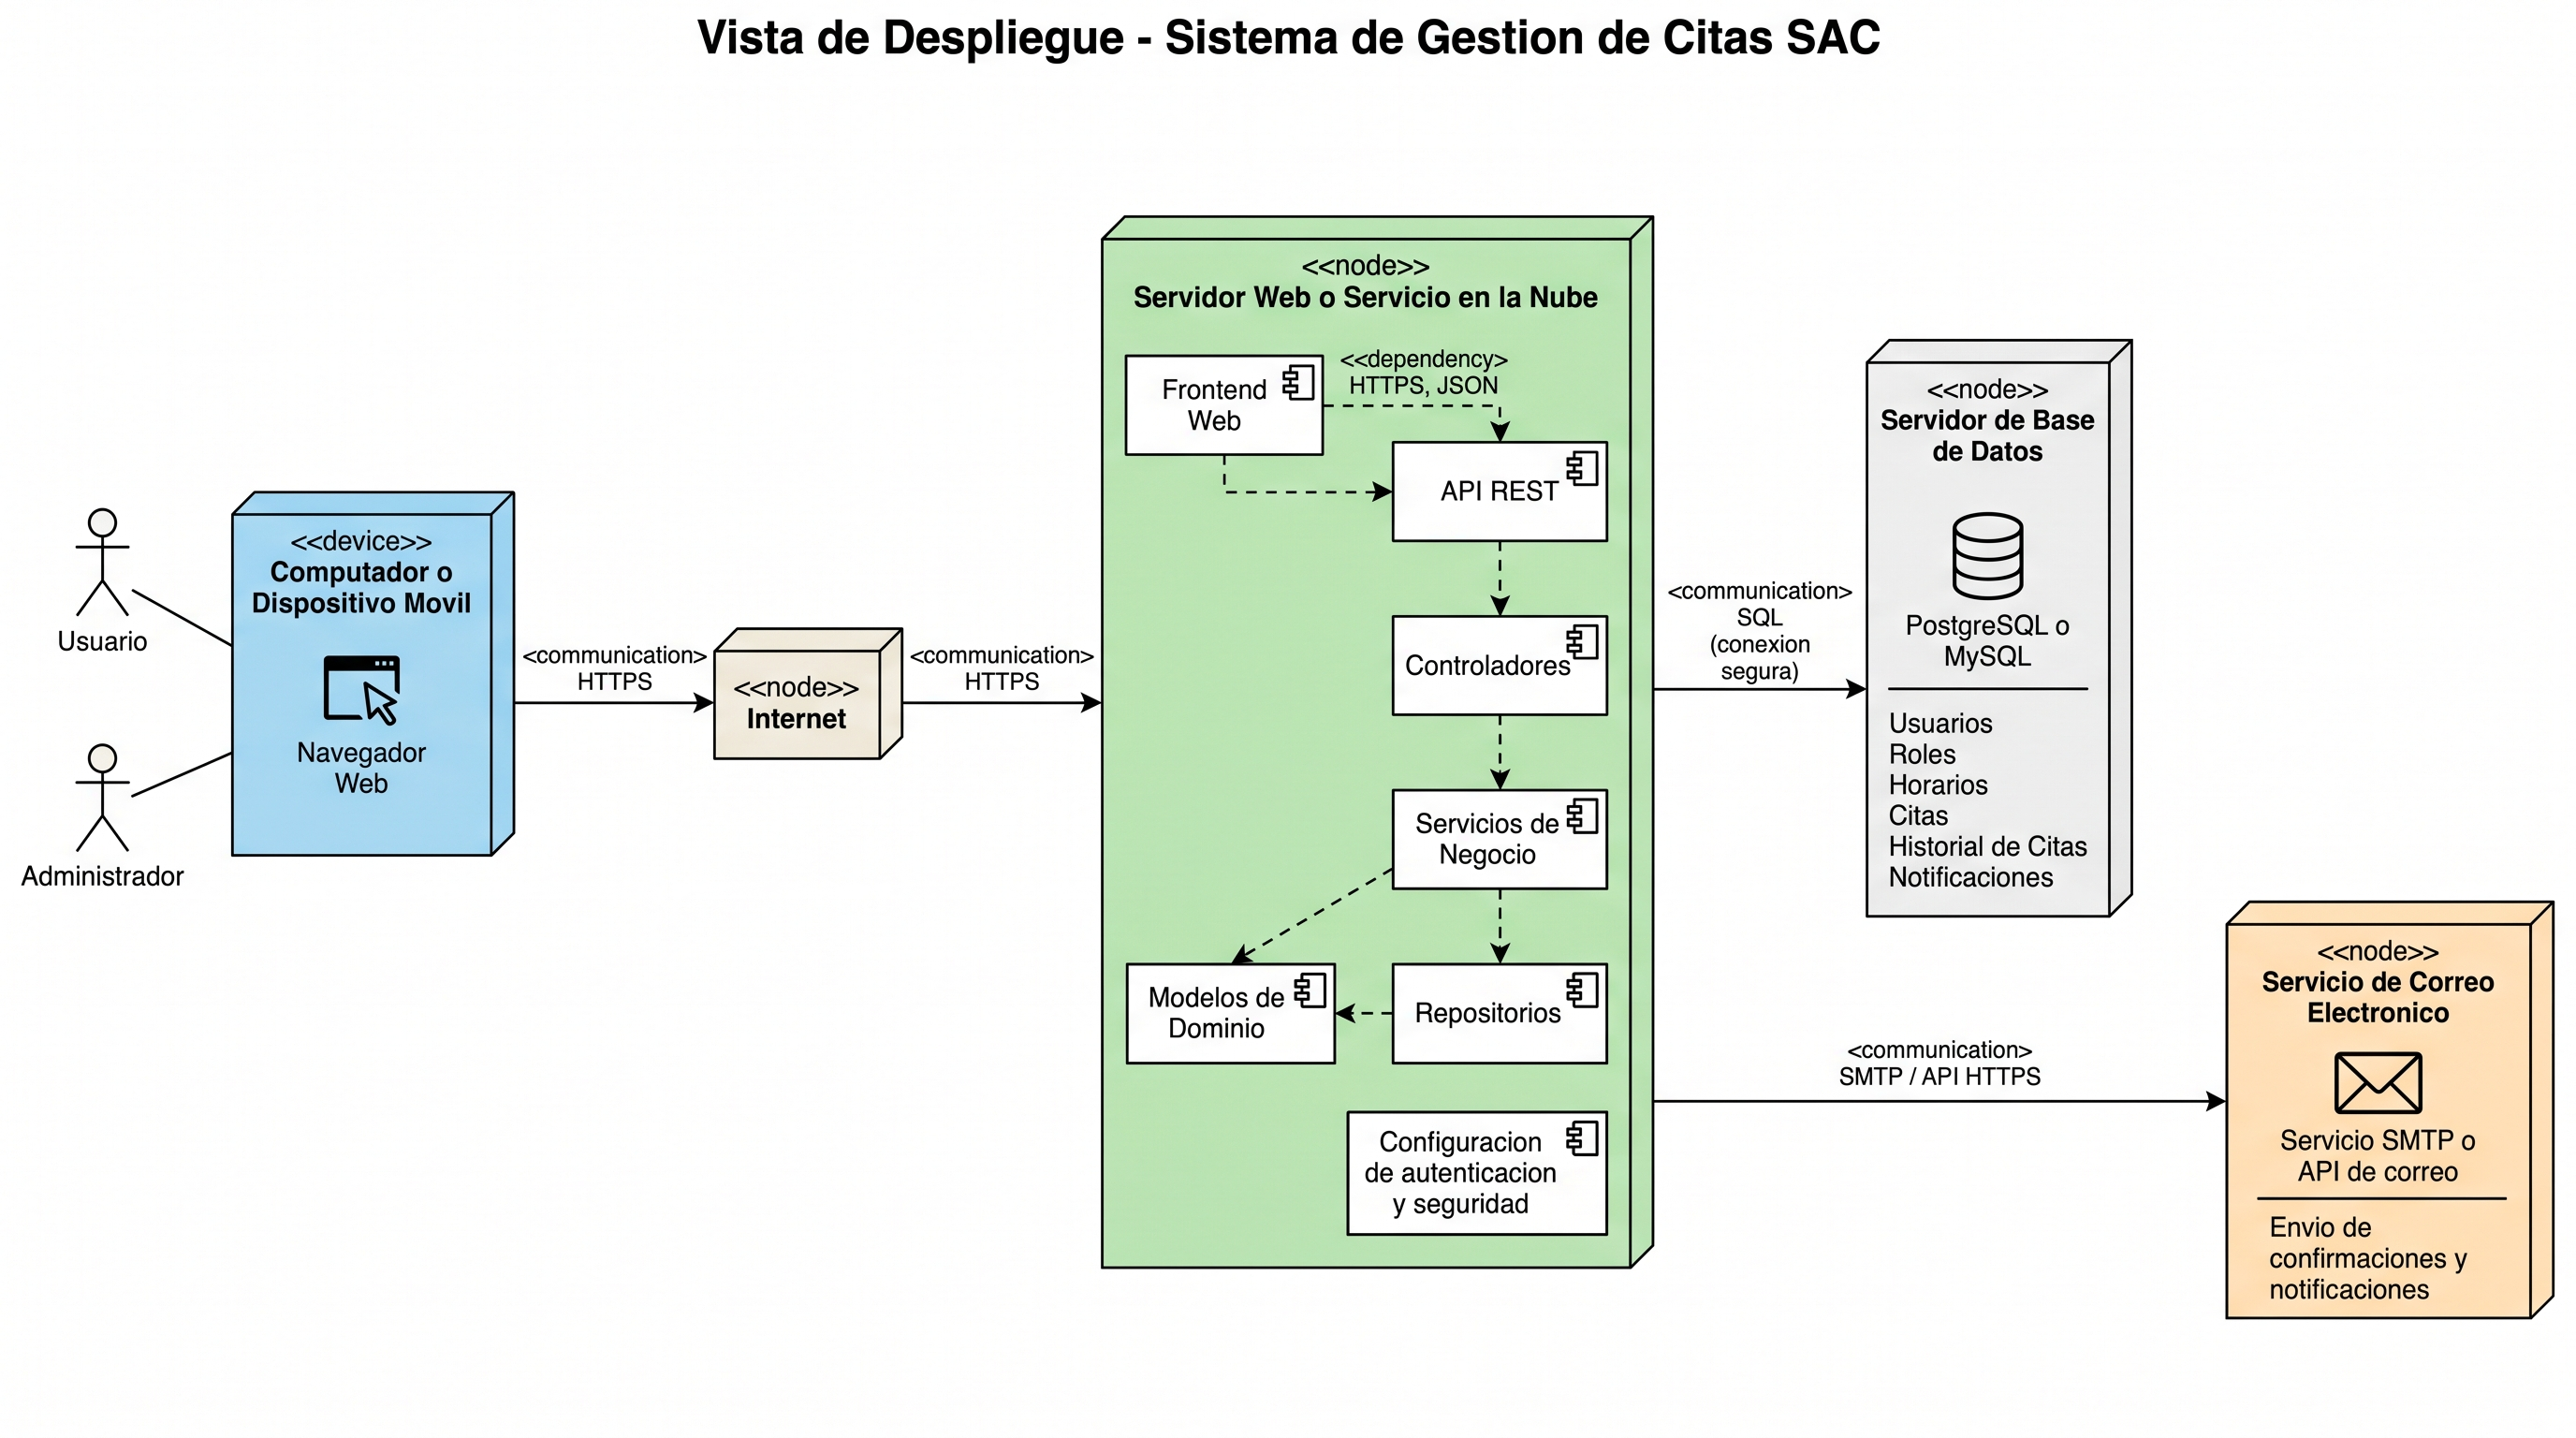
\includegraphics[width=0.9\textwidth]{diagrama_despliegue_sac.jpg}
    \caption{Vista de despliegue del Sistema de Gestion de Citas SAC.}
    \label{fig:despliegue-sac}
\end{figure}


En la Figura~\ref{fig:despliegue-sac} se representa que el usuario o administrador accede desde un computador o dispositivo movil mediante un navegador web. La comunicacion se realiza por Internet utilizando HTTPS, lo que permite proteger la informacion transmitida.

El servidor web o servicio en la nube aloja el frontend, la API REST, los controladores, los servicios de negocio, los modelos de dominio y los repositorios. Este servidor se conecta de manera segura con el servidor de base de datos, donde se almacenan usuarios, roles, horarios, citas, historiales y notificaciones. Finalmente, el sistema se comunica con un servicio externo de correo electronico para enviar mensajes relacionados con las citas.

\section{Herramientas para optimizar el desarrollo}

La arquitectura propuesta requiere herramientas que apoyen la construccion, prueba, control de cambios, documentacion y despliegue del sistema.

\begin{longtable}{|p{3.3cm}|p{4cm}|p{6.7cm}|}
\hline
\textbf{Necesidad} & \textbf{Herramienta propuesta} & \textbf{Uso dentro del proyecto} \\
\hline
\endfirsthead
\hline
\textbf{Necesidad} & \textbf{Herramienta propuesta} & \textbf{Uso dentro del proyecto} \\
\hline
\endhead
\hline
\endfoot
\hline
\endlastfoot

Entorno de desarrollo & Visual Studio Code & Edicion de codigo, terminal integrada, extensiones, Git y ejecucion de tareas del proyecto. \\
\hline

Backend & Python con FastAPI o Django & Implementacion de API REST, validaciones, autenticacion, logica de negocio y principios POO. \\
\hline

Frontend & HTML5, CSS3 y JavaScript & Construccion de formularios, paneles, agenda y experiencia responsiva para usuario y administrador. \\
\hline

Base de datos & PostgreSQL o MySQL & Almacenamiento persistente de usuarios, roles, horarios, citas, historial y notificaciones. \\
\hline

Control de versiones & Git y GitHub & Historial de cambios, respaldo del codigo, ramas de trabajo y documentacion de evidencias. \\
\hline

Modelado y arquitectura & Draw.io & Creacion de diagramas UML de clases, componentes, despliegue, casos de uso y actividades. \\
\hline

Pruebas de API & Postman & Envio de solicitudes HTTP, validacion de endpoints y documentacion de colecciones de prueba. \\
\hline

Pruebas automatizadas & Pytest & Verificacion de servicios, validaciones, reglas de negocio y resultados esperados. \\
\hline

Dependencias Python & requirements.txt & Centralizacion de librerias necesarias para instalar y ejecutar el proyecto de manera repetible. \\
\hline

Contenedores & Docker & Empaquetado de aplicacion, base de datos y dependencias para mantener consistencia entre entornos. \\
\hline

Despliegue & VPS o plataforma en la nube & Publicacion de la aplicacion para permitir acceso remoto y administrar disponibilidad. \\
\hline

Documentacion & LaTeX y Markdown & Elaboracion de informes academicos, manuales, guias tecnicas y documentacion del repositorio. \\
\hline
\end{longtable}

La seleccion de estas herramientas permite optimizar el proceso de desarrollo. Visual Studio Code, Git y GitHub facilitan el trabajo diario y el control de cambios. Draw.io ayuda a documentar la arquitectura. Postman y Pytest apoyan la validacion de funcionalidades. Docker y una plataforma en la nube permiten que la aplicacion pueda desplegarse de manera consistente en diferentes ambientes.

\section{Beneficios de la arquitectura propuesta}

La arquitectura seleccionada ofrece los siguientes beneficios para el Sistema de Gestion de Citas SAC:

\begin{itemize}[leftmargin=1.2cm]
    \item Facilita el mantenimiento al separar interfaz, controladores, servicios, modelos y repositorios.
    \item Reduce la duplicacion de reglas de negocio al centralizarlas en servicios especializados.
    \item Mejora la seguridad al controlar autenticacion y roles desde la capa de API y servicios.
    \item Permite probar los componentes de forma aislada, especialmente servicios y repositorios.
    \item Facilita ampliar la aplicacion con nuevos modulos, como reportes, recordatorios o integraciones externas.
    \item Permite cambiar detalles de infraestructura, como la base de datos o el servicio de correo, con menor impacto sobre la logica principal.
    \item Favorece la trazabilidad de las citas mediante historial de cambios y notificaciones.
    \item Permite desplegar la aplicacion en una infraestructura escalable y accesible desde diferentes dispositivos.
\end{itemize}

\section{Conclusiones}

La arquitectura de software propuesta para el Sistema de Gestion de Citas SAC se basa en una estructura web por capas que separa la presentacion, la API, la logica de negocio, el dominio, la persistencia y los servicios externos. Esta organizacion permite que cada componente tenga una responsabilidad definida y facilita el mantenimiento de la aplicacion.

El patron MVC permite separar la interfaz de usuario de los modelos y controladores. Los patrones Service Layer y Repository complementan esta arquitectura al centralizar las reglas del negocio y encapsular el acceso a datos. Adicionalmente, Factory Method y Observer apoyan la creacion y envio de notificaciones relacionadas con cambios de estado de las citas, mientras que DTO permite transferir datos controlados entre el frontend y la API.

La vista de componentes permite comprender como se relacionan el frontend, la API, los controladores, los servicios, los repositorios y la base de datos. La vista de despliegue muestra las condiciones tecnicas necesarias para implantar la solucion, incluyendo dispositivos cliente, Internet, servidor de aplicacion, base de datos y servicio de correo externo.

Finalmente, la seleccion de herramientas como Visual Studio Code, Python, PostgreSQL, GitHub, Draw.io, Postman, Pytest y Docker contribuye a optimizar el ciclo de desarrollo. En conjunto, la arquitectura propuesta permite construir una solucion organizada, segura, escalable y coherente con las necesidades del Sistema de Gestion de Citas SAC.

\end{document}
